\subsection{Product perspective}
\subsubsection{Technologies overview}
\begin{itemize}
\item Android Studio Development Kit
\begin{itemize}
\item Kotlin
\item Android Compose
\end{itemize}
\item Data management
\begin{itemize}
\item Google Firestore
\item Google Firebase
\item Database
\item Room
\item Shared preferences
\end{itemize}
\item Authentication
\begin{itemize}
\item Google Authentication
\item Facebook Authentication
\item Email Authentication
\end{itemize}
\item External APIs
\begin{itemize}
\item Google Maps
\item Google Translate
\item Google Cloud Messaging
\item Google Places
\item OpenWeatherMap
\item GPT 3 - OpenAI
\end{itemize}
\end{itemize}
\newpage
\subsubsection{Internal structure}
\hspace{\parindent}The proposed system uses an application on the server side that is connected with the APIs to the Android on the phone. 

The Way of communication between the parts of the system and logic behind the system is presented in the following figure:

\begin{figure}[!htb]
\centering
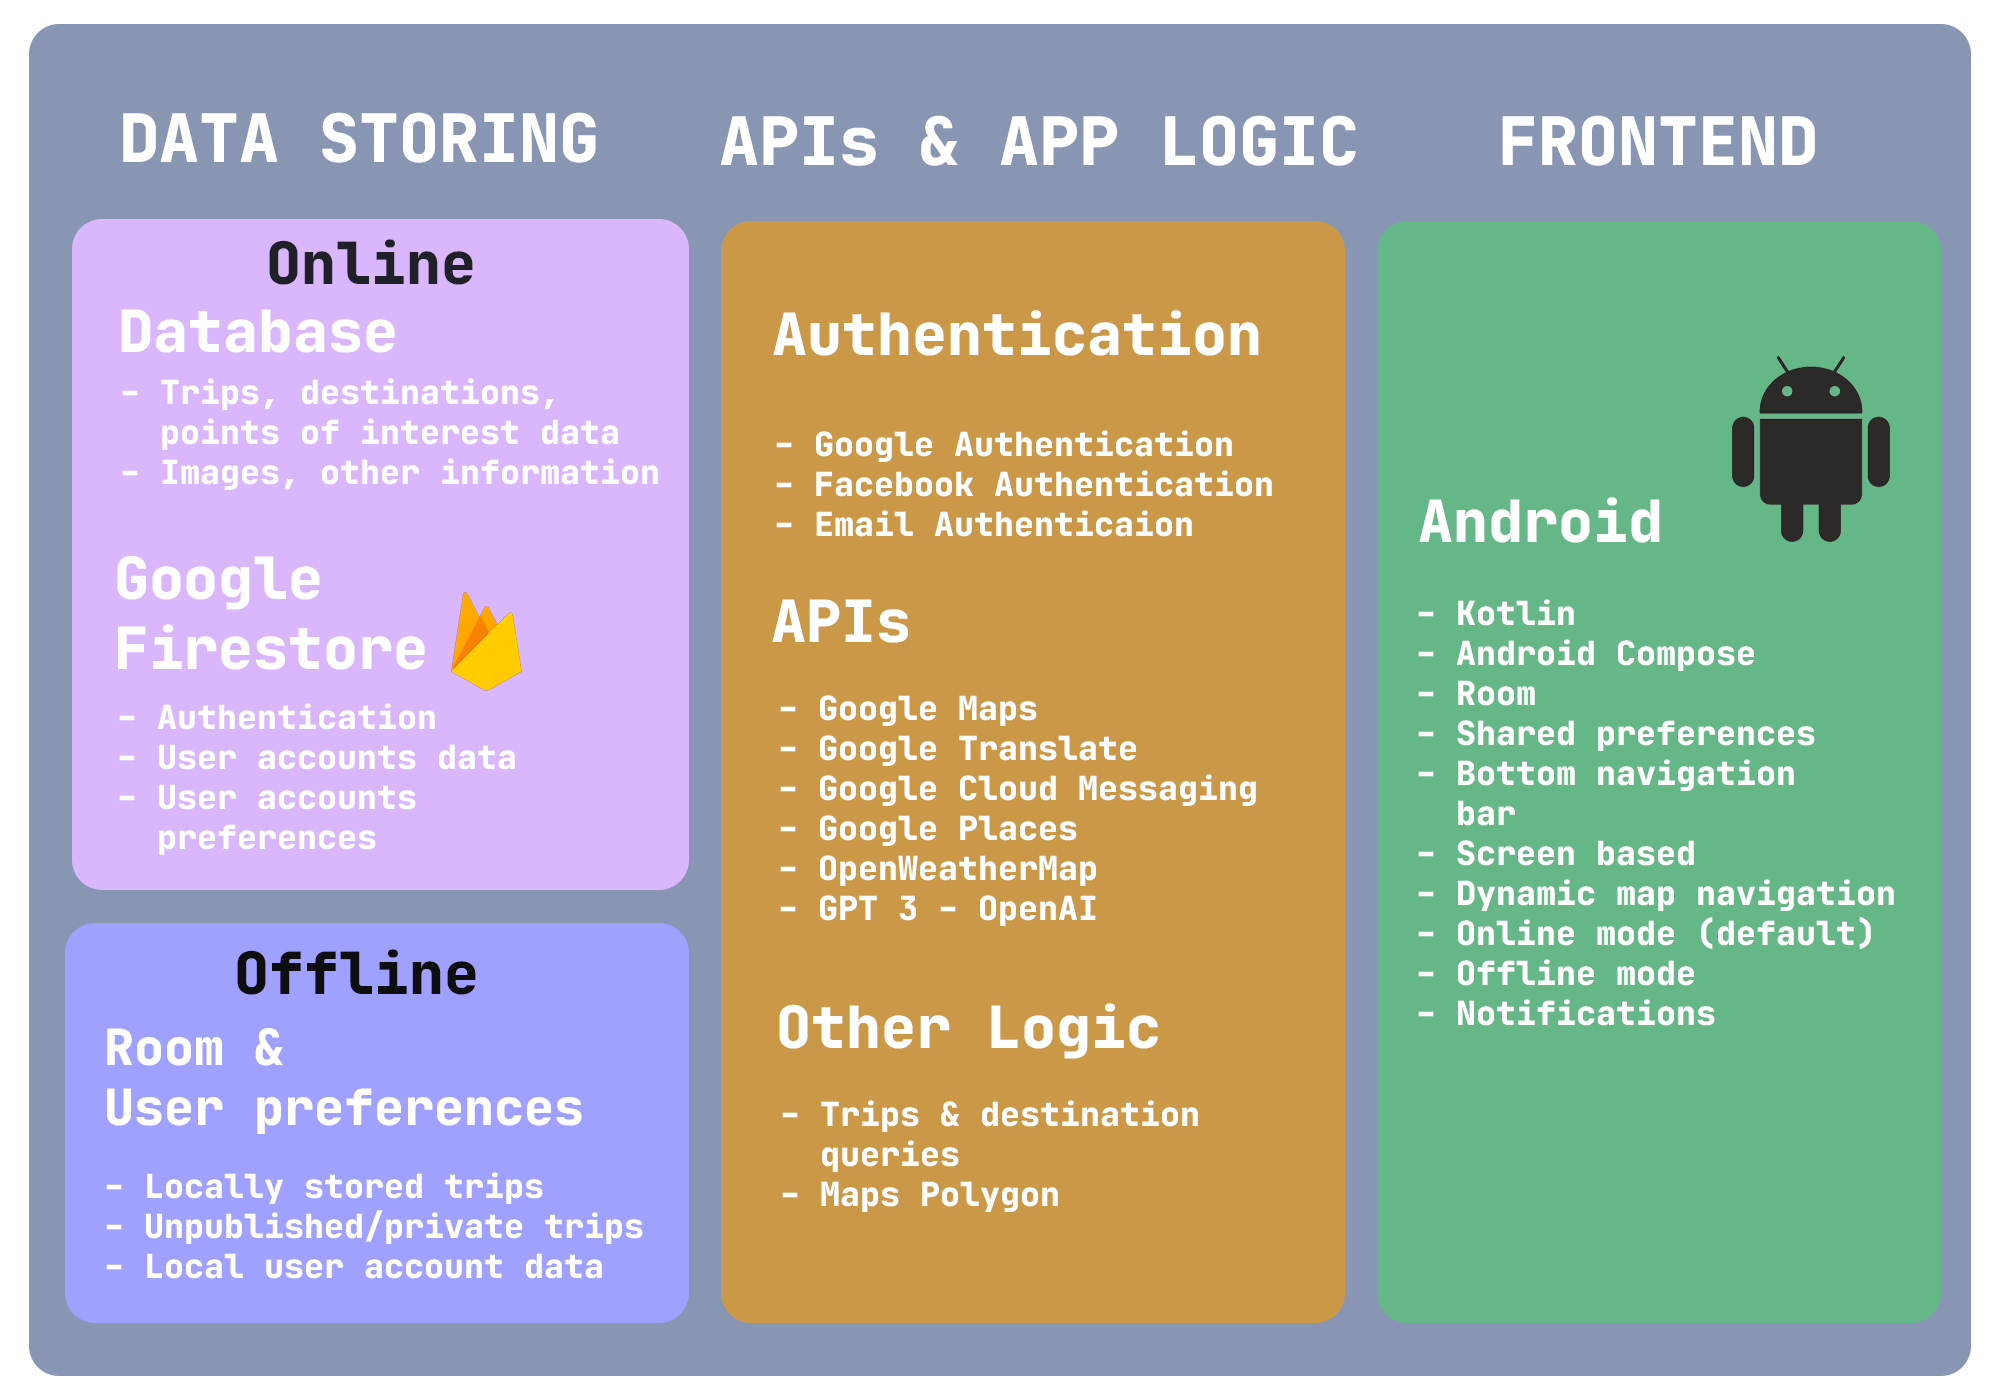
\includegraphics[width=\textwidth]{../Images/InternalStructurePNG_v2.png}
\caption{\label{fig:dbapiuser}\textbf{Internal structure of the system}}
\end{figure}

\textbf{Data storing}\\

The database part is divided into two separate entities. Most of the authentication part is done directly through Google Firebase and Firestore frameworks, which offer great support for Google and Facebook accounts login integration, as well as native support for email based accounts. Controlling authentication via Google services is fast, easy, and seamless, so we have decided to keep most of our logic, as well as account data, stored here. \\ \\
User account details, such as username, ID, and user preferences, are stored in the Google Firestore database, and are fetched after every login, so that the local user account data is consistent with the one on the servers. \\ \\
Images that are used for trips and destinations are also stored in the Google Firestore database.\\ \\
The other part of the database, which stores the data about the destinations, trips, points of interests, and other features related directly to the workflow of the app, are stored in another, separate database. This decision was due to the fact that Google Firestore is a NoSQL database, so putting relational data there would make it inefficient and slow compared to the traditional SQL database.\\ \\
This is what made us decide to transfer this data to completely other place and use a different technology than with the accounts. Account data storing and fetching works exceptionally well and fast with Google services, so we had no real reason to move it from there, especially since that data is more sensitive and Google services provide high level of protection. \\ \\
Android framework also supports numerous features for working locally. We have used these features to have an additional "offline" mode of our application, which allows full functionalities despite the user not having internet connection. We use Android Room to store all the desired trips downloaded and edited by the user, as well as the ones that the user has created locally and decided not to publish yet. "Offline" mode is then synced as soon as the user gets Internet connection, if any additional changes have been made to the local or public trips. \\ \\
Finally, shared preferences are used to store the user's local information such as username, theme preferences, display name, and other features that help user while navigating the app. These are updated with the data located in the Google Firestore framework.\\
\\

\textbf{APIs \& App Logic}\\

Authentication used for the application is done directly through Google Firbase. Account creation can be done directly through email, after which it has to be confirmed via confirmation email. The other way of creating account is logging in with either Facebook or Google account. This way account gets automatically created, or joined if it has already been previously created with the same email. This allows users to not have to worry with which account they have logged in before, as it is all connected to the same email. Users would have to be logged in to either their Google or Facebook account before using those methods to log in to the app.\\ \\
Google and Facebook "button" directly communicate with their respective APIs and only after the conversation has successfully ended do communicate with Google Firebase servers. \\ \\
Another thing that is used from Google framework is the Google Maps API. From that API, several different features are used, such as Maps presentation, location searching, cities searching, distance calculation, and others. Google Maps are dynamically presented in the app and allow users to search through them either by text or by touch.\\ \\
Another important thing is a small PHP script that is running on the server. It serves as a backend of the app, handling query fetching, control, and execution, as well as handling and displaying data that is coming and going through Google Maps API.\\ \\ 
This PHP script is returning all the necessary data in the form of JSON files, which are then handled by the app accordingly and to its needs.

\textbf{Frontend}\\

On the frontend side, we have decided to use all of the latest technologies recommended by Google for Android app development. \\ \\
Kotlin is used as the programming language, which allows better data and variable control in Android environment than the previous official language Java.\\ \\
From the pure design perspective, Android Compose is used instead of the previous template/xml based design. Compose allows for creation of certain elements, as well as their dynamic modelling, which allows for reusability and code cleanliness. Compose allows for elements to by dynamically inserted into specific places, as well as to be dynamically changed, hidden, or manipulated in a much faster and easier fashion. It also allows for faster development since the previews of those compose components can be rendered much faster.\\ \\
As the base of the system, bottom bar with different pages has been used. More on that part is explained in latter chapters of this document.
\\ \\ 
The app supports both online and offline mode, with shared preferences used for storing local display preferences of the app.\\ \\
\newpage

\subsubsection{Scenarios}

\textbf{Scenario 1}\\

\hspace{\parindent}Marco wants to go to a trip to France. His friend, Federico, already went on a trip in a similar area and visited points of interest that Marco likes. Marco asked Federico to tell him all of the places he visited, how did he travel, and the order in which he visited these places. Federico made some notes for Marco, but it still left Marco with the problem of having everything in his phone organized and in one place. That's when Marco found out about the app and asked Federico to put everything he remembers from the trip here. That way Marco had all of the locations in the correct order, as well as comments about certain places and other detailed information all in one place, which allowed him to easier follow the trip during his time in France.\\

\textbf{Scenario 2}\\

\hspace{\parindent}Rebecca, the friend of Marco and Federico, heard about their trip to France and decided to go there as well. However, she is not as interested into visiting so many French castles like Marco and Federico, and wants to add some other destinations to her trip. However she still wants to keep the first half of the trip, where guys visited the southern part of France. She also uses the app and copies the trip, after which she edits it and replaces castle destinations with beaches on the northern part of the country. She renames the trip and publishes it with a different name. This way Rebecca saved some time and effort on planning the entire first half of the trip, whilst being able to modify the experience in the latter half.\\

\textbf{Scenario 3}\\

\hspace{\parindent}Giovanna wants to on a trip but she already visited France. She needs some new ideas. By using the "explore" function in the app she finds some of the top rated trips around Europe - her favourite of those is a trip to Iceland. Giovanna follows all of the guidelines in the trip and has an amazing time.\\

\subsection{Product functions}
\hspace{\parindent}Functions of the system provide easy and intuitive ways to use the app. They are somewhat connected and have overlapping features. Nevertheless, the users may use only certain parts of the system and still get the full functionality they need from the app.
These functions are mentioned in several places in the document, but their most thorough explanation can be found here.
\subsubsection{Adding a trip}
\hspace{\parindent}Adding a trip is the most essential part of the system. The function features several parameters and allows for high level of customizability in order to create a fully unique travel experience. \\
Each point of interest is featured as a specific "destination", although even places that are not regarded as specific destinations can be inserted into a trip. Destination fetching is done through the Google Maps API, with the users also having the ability to add and edit their own destinations.
The function features the following:
\begin{itemize}
\item Selecting a starting point, that is then connected to the nearest city on the map
\item Adding other destinations to the trip
\item Writing a trip description
\item Adding preferred way of travel between destinations
\item Identifying trip price level
\item Adding comments to trip destinations
\item .............
\end{itemize}
\subsubsection{Editing a trip}
\hspace{\parindent}Editing a trip can be done on two different types of trips - public or private. If the trip is public, either published by the user editing it or someone else, by starting to editing an exact copy of that trip is created, which can then be published again under different name and different trip ID.\\
If the trip is private and has not yet been published, then a new trip is not created, but rather the trip ID stays the same. If the trip is then published and edited again, the new edited version of the trip has a new trip ID and is a whole new entity.\\
Editing a trip features all of the same functions that adding a trip does, which means that everything from a small comment to the whole trip can be changed. 
\subsubsection{Finding a trip}
\hspace{\parindent}Finding a trip can be done in several different ways. The first way features a search bar which then searches a trip by the starting point name or by the city which is the closest to that destination. The second way is a search by the trip ID or a hyperlink, which can be directly received from other users. The third way is by accessing a specific user's account page and scrolling through their published trips. Finally, trips can also be found by looking at the interactive map, selecting the area of the desired starting point of the trip, and finding the trip through the distinct trip name and photo.  
\subsubsection{Following a trip}
\hspace{\parindent}This function mainly uses a specific trip and sets it as an active trip of the user. This makes it easily accessible by the user at all times by using the bottom navigation bar, and allows him to follow certain steps of the trip without losing progress. This function also allows the user to change the current active trip and still keep the progress of an old trip, so that the progress can be easily restored when that trip is again set as an active trip.
\subsubsection{Updating account settings}
\hspace{\parindent}Only a few settings can be changed in the user account. List is the following:
\begin{itemize}
\item Changing a username
\item Changing a profile picture
\item Switching between dark and light colour scheme
\item Setting preferred price level
\item Switching between offline mode and online mode
\end{itemize}
\subsubsection{Offline function}
\hspace{\parindent}The system allows the users to be disconnected from the Internet and still use the app fully. Individual trips can be downloaded and store in the phone internal storage, and then accessed at any time. If any changes are made to the trip during the offline time, a new iteration of the trip gets created and published as soon as the connection is restored and the user has come back to the online mode. Multiple trips can be downloaded and kept in the storage of the phone at all times.  
\subsection{Additional features}
\subsubsection{Translation}
\hspace{\parindent}Translation API is used to translate some information about the trips. The app will detect the language of the phone and translate the description of a specific trip to this language. This allows users to quickly see the overview of the trip and decide whether they like it or not, as the app is meant to be used on the international level, it is highly possible that a large number of users will not use English as their primary language.
\subsubsection{Multiple language support}
\hspace{\parindent}Besides the translating descriptions, the app offers a variety of different languages in which it can be used. Every single function and word in the app is translated into the language of the system, and is completely usable without needing to know a single word of English language. The app currently supports only two additional languages, Italian and Croatian, to go along with the original English, but the infrastructure is set so that more languages can be added swiftly and easily.


